\documentclass{standalone}
\pagestyle{empty}
\usepackage{tikz}
\usetikzlibrary{arrows.meta,bending}

\begin{document}
\noindent
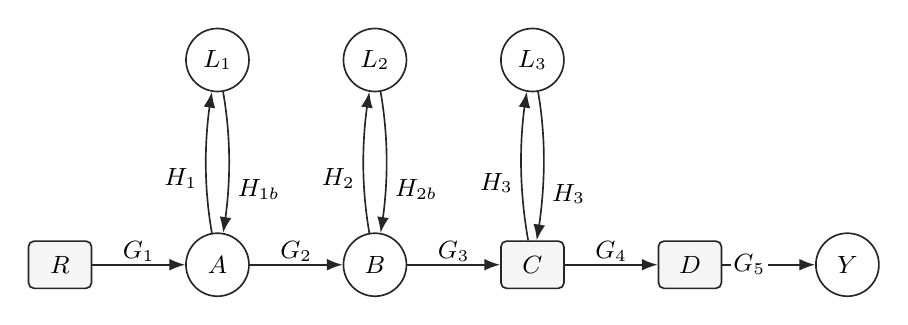
\begin{tikzpicture}[
  >=Latex,
  ->,
  semithick,
  every node/.style={font=\small},
  signal node/.style={circle,draw,minimum size=8mm,inner sep=1pt,fill=white},
  io node/.style={rectangle,rounded corners=2pt,draw,minimum width=8mm,minimum height=6mm,inner sep=2pt,fill=gray!8},
  every path/.style={draw=black!85},
  edge label/.style={fill=white,inner sep=1pt,text=black},
]
\node[io node] (R) at (0.0,0.0) {$R$};
\node[signal node] (A) at (2.0,0.0) {$A$};
\node[signal node] (B) at (4.0,0.0) {$B$};
\node[io node] (C) at (6.0,0.0) {$C$};
\node[io node] (D) at (8.0,0.0) {$D$};
\node[signal node] (Y) at (10.0,0.0) {$Y$};
\node[signal node] (L1) at (2.0,2.6) {$L_1$};
\node[signal node] (L2) at (4.0,2.6) {$L_2$};
\node[signal node] (L3) at (6.0,2.6) {$L_3$};
\draw (R) -- node[edge label,midway,above] {$G_1$} (A);
\draw (A) -- node[edge label,midway,above] {$G_2$} (B);
\draw (B) -- node[edge label,midway,above] {$G_3$} (C);
\draw (C) -- node[edge label,midway,above] {$G_4$} (D);
\draw (D) -- node[edge label,midway,left] {$G_5$} (Y);
\draw (A) to[out=100,in=260,looseness=0.85] node[edge label,pos=0.35,left,xshift=-2pt,yshift=2pt] {$H_1$} (L1);
\draw (L1) to[out=280,in=80,looseness=0.85] node[edge label,pos=0.65,right,xshift=2pt,yshift=-2pt] {$H_{1b}$} (A);
\draw (B) to[out=100,in=260,looseness=0.85] node[edge label,pos=0.35,left,xshift=-2pt,yshift=2pt] {$H_2$} (L2);
\draw (L2) to[out=280,in=80,looseness=0.85] node[edge label,pos=0.65,right,xshift=2pt,yshift=-2pt] {$H_{2b}$} (B);
\draw (C) to[out=100,in=260,looseness=0.85] node[edge label,pos=0.35,left,xshift=-2pt,yshift=2pt] {$H_3$} (L3);
\draw (L3) to[out=280,in=80,looseness=0.85] node[edge label,pos=0.65,right,xshift=2pt,yshift=-2pt] {$H_{3}$} (C);
\end{tikzpicture}
\end{document}
